\section{IMPLEMENTATION}


	 \subsection{Approach}
	
		The implementation of our project was structured into several distinct phases, each centered around specific gameplay mechanics, visual design, and user interaction. This approach facilitated a continuous process of refinement and enhancement as we progressed.
	
	 \subsubsection{Tools and Technologies}
		\begin{enumerate}
			\item Programming Languages
					We selected C++ as the primary programming language for our game's development. Its exceptional speed and object-oriented nature significantly streamlined the process of coding the game's mechanics.
			\item Libraries
					For multimedia and graphics user interface implementation, we harnessed the capabilities of the SFML library. Chosen for its user-friendly syntax and comprehensive toolkit, SFML provided us with all the essential resources required for effective game development.
			
		\end{enumerate}
	
	\subsubsection{System Architecture and Design}
	
		The architecture of "Baal Arjun" was thoughtfully structured to ensure both flexibility and scalability. Key components encompassed in this architecture include:
		
		\begin{enumerate}
			\item Player Controller:
				Responsible for managing player inputs, character movement, and shooting mechanics.
			
			\item Enemy Automation:
				Incorporating dynamic enemy movement and     arrow-shooting behavior.
			
			\item Collision Detection: 
				 Overseeing accurate collision detection between arrows, characters, and the game environment.
				 
			\item Level Implementation:
					Designing and integrating game levels to ensure a dynamic player experience.
			\item User Interface (UI):
					 Displaying essential in-game information such as health, arrow count, and visual elements for enemies and player arrows.
			\item Sound Implementation:
					Enriching gameplay through auditory elements.
			
		\end{enumerate}
		
 \subsubsection{Code Development}
			
			The foundational gameplay mechanics were meticulously developed, spanning aspects like player movement, arrow physics, enemy behavior, shooting mechanisms, collision detection, and the implementation of diverse game levels. Algorithmic solutions were devised for trajectories of normal and Sudarshan arrows, each rigorously tested and refined. Emphasis was placed on crafting self-documented code, achieving modularity for code reusability.
	
	 \subsubsection{Resource Collection}
	
	 		Resources such as images, sounds, and fonts were thoughtfully curated from online sources. Furthermore, Adobe Illustrator was leveraged to modify these resources to align precisely with our project's creative vision.
	 		
	 		
	  \subsubsection{Integration and Testing}
	 
	 		The integration process commenced by combining shooting algorithms with collision detection algorithms, subjecting them to comprehensive testing to ensure their seamless functionality. Concurrently, the graphical user interface (GUI) underwent development. Eventually, the GUI and game logic converged into the final cohesive product. A testing phase was initiated, involving friends as testers who aided in identifying and rectifying any bugs encountered.
	 		
	 \subsubsection{ Version Control and Collaboration}
	 
	 		To facilitate seamless collaboration, GitHub served as our chosen version control system. Regular code synchronization was achieved through Git, ensuring that contributions from all team members were harmoniously integrated.
	 		


This comprehensive implementation phase not only actualized our project but also exemplified our commitment to precision, collaboration, and the realization of an engaging gaming experience.

\newpage
\subsection{Flow Chart}

\vspace{2cm}
\begin{figure}[h]
	
	\centering
	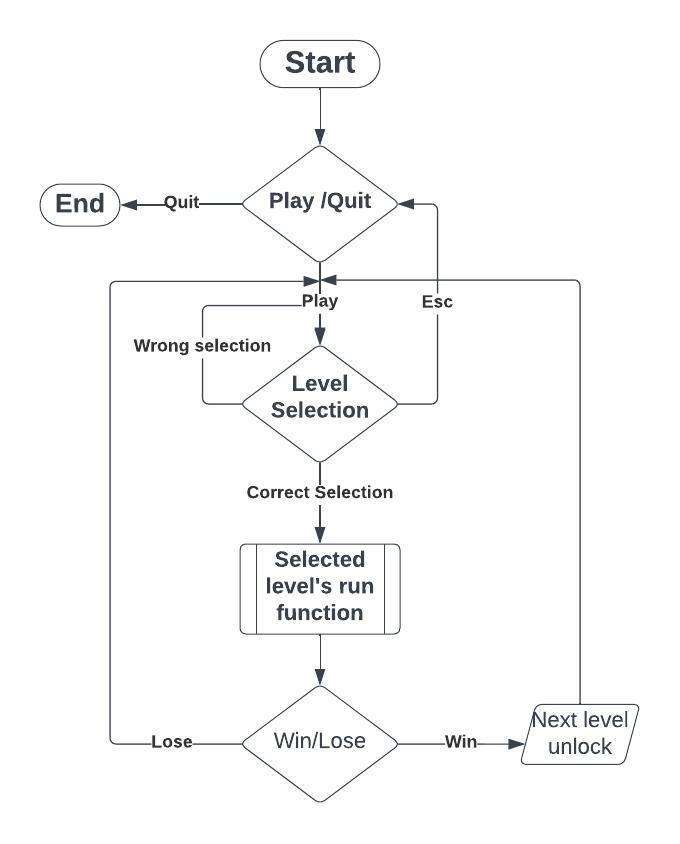
\includegraphics{sec/pdf/flowchart}
	\caption{Flow Chart}
\end{figure}

\newpage
\subsection{Block Diagram}

\vspace{2cm}
\begin{figure}[h]
	
	\centering
	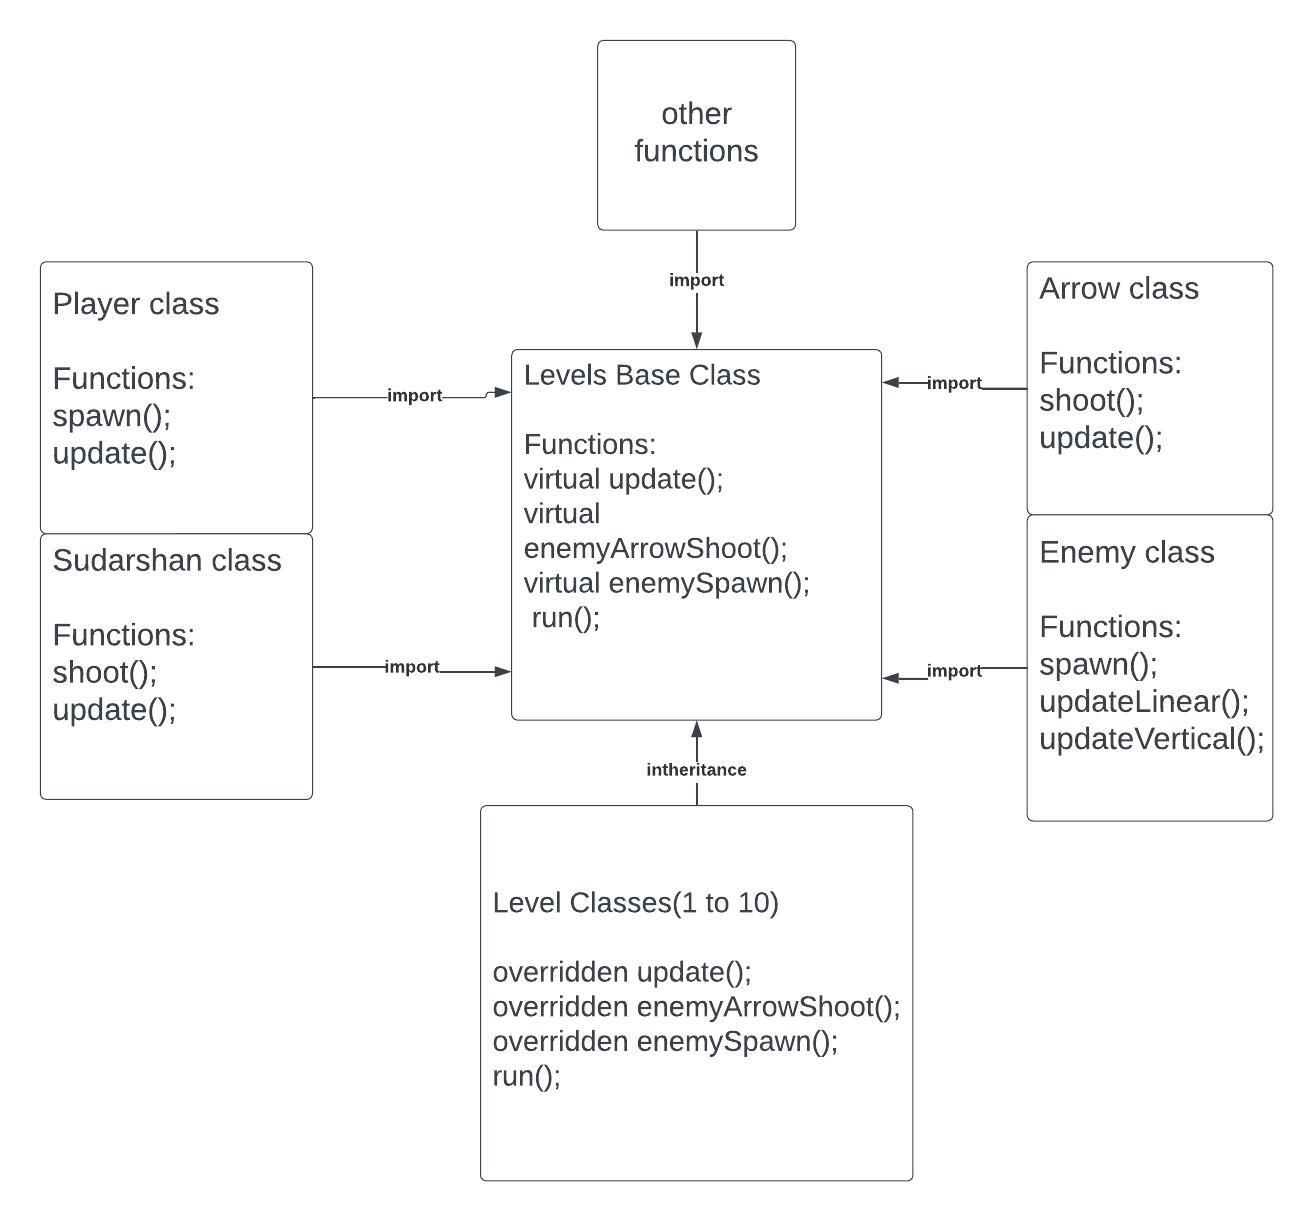
\includegraphics[width = \textwidth]{sec/pdf/blockDiagram}
	\caption{Generalized Block Diagram}
\end{figure}

\newpage
\subsection{Game Pictures}
\vspace{2cm}
\begin{figure}[h]
	
	\centering
	
\includegraphics[width = \textwidth]{sec/pdf/main}
	\caption{Main Screen}
\end{figure}
\vspace{2cm}
\begin{figure}[h]
	
	\centering
	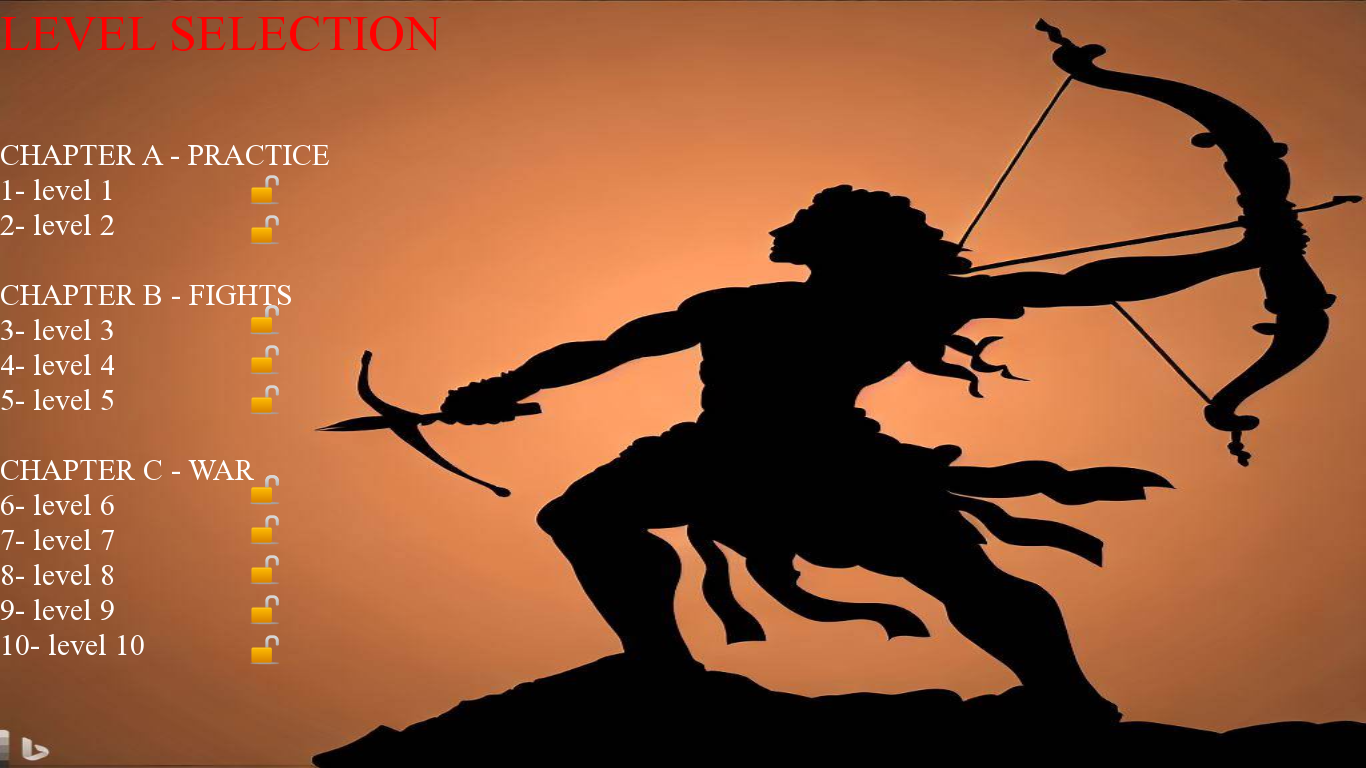
\includegraphics[width = \textwidth]{sec/pdf/chapters}
	\caption{Level Selection Screen}
\end{figure}

\newpage
\begin{figure}[h]
	
	\centering
	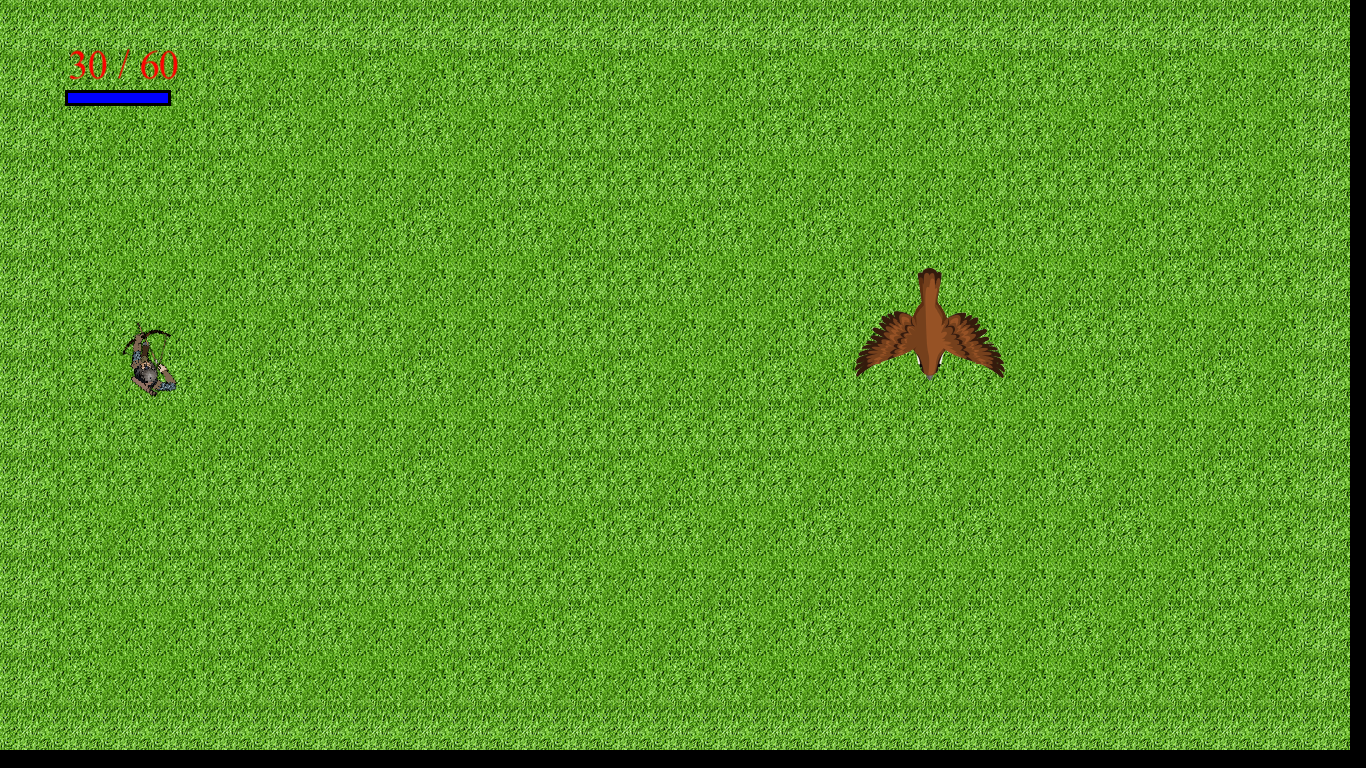
\includegraphics[width = \textwidth]{sec/pdf/level2}
	\caption{Level 2}
\end{figure}
\vspace{2cm}
\begin{figure}[h]
	
	\centering
	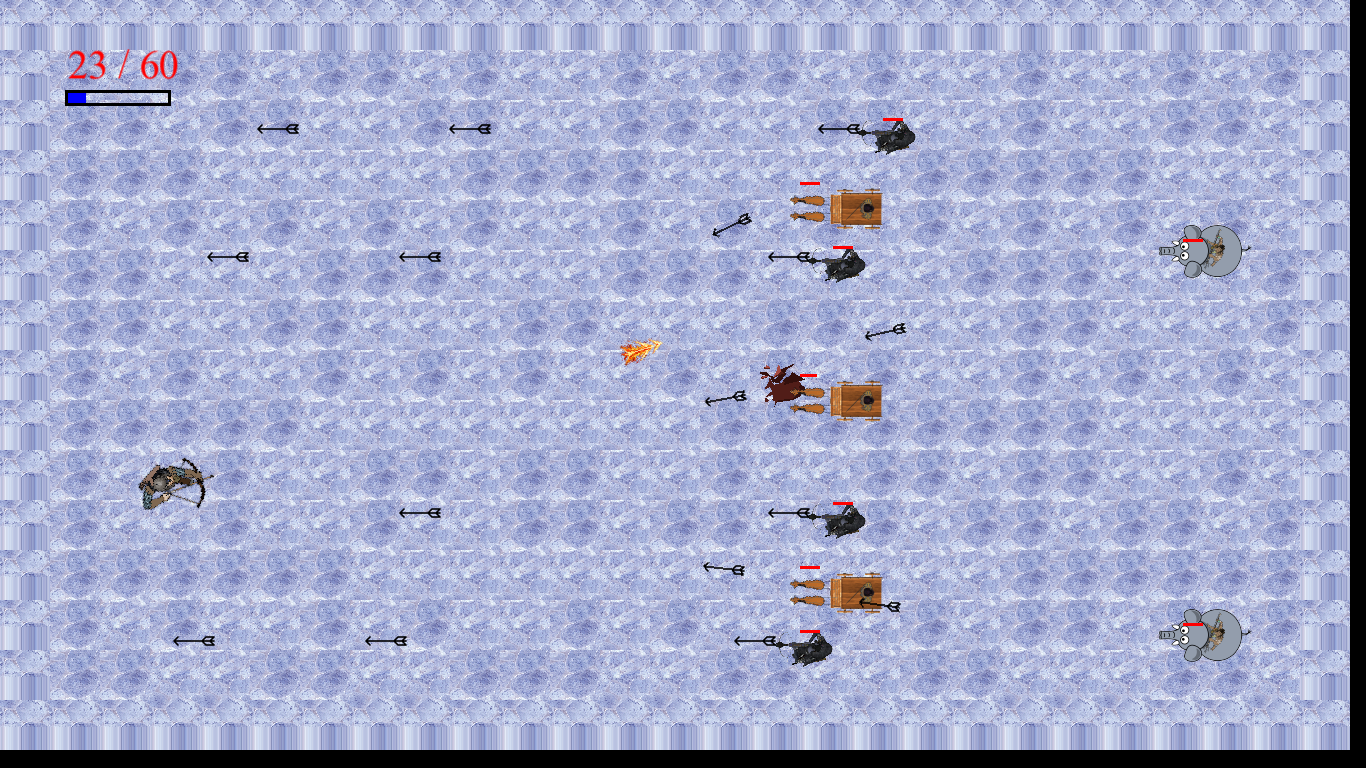
\includegraphics[width = \textwidth]{sec/pdf/level 7}
	\caption{Level 7}
\end{figure}
\newpage
\vspace{2cm}
\begin{figure}[h]
	
	\centering
	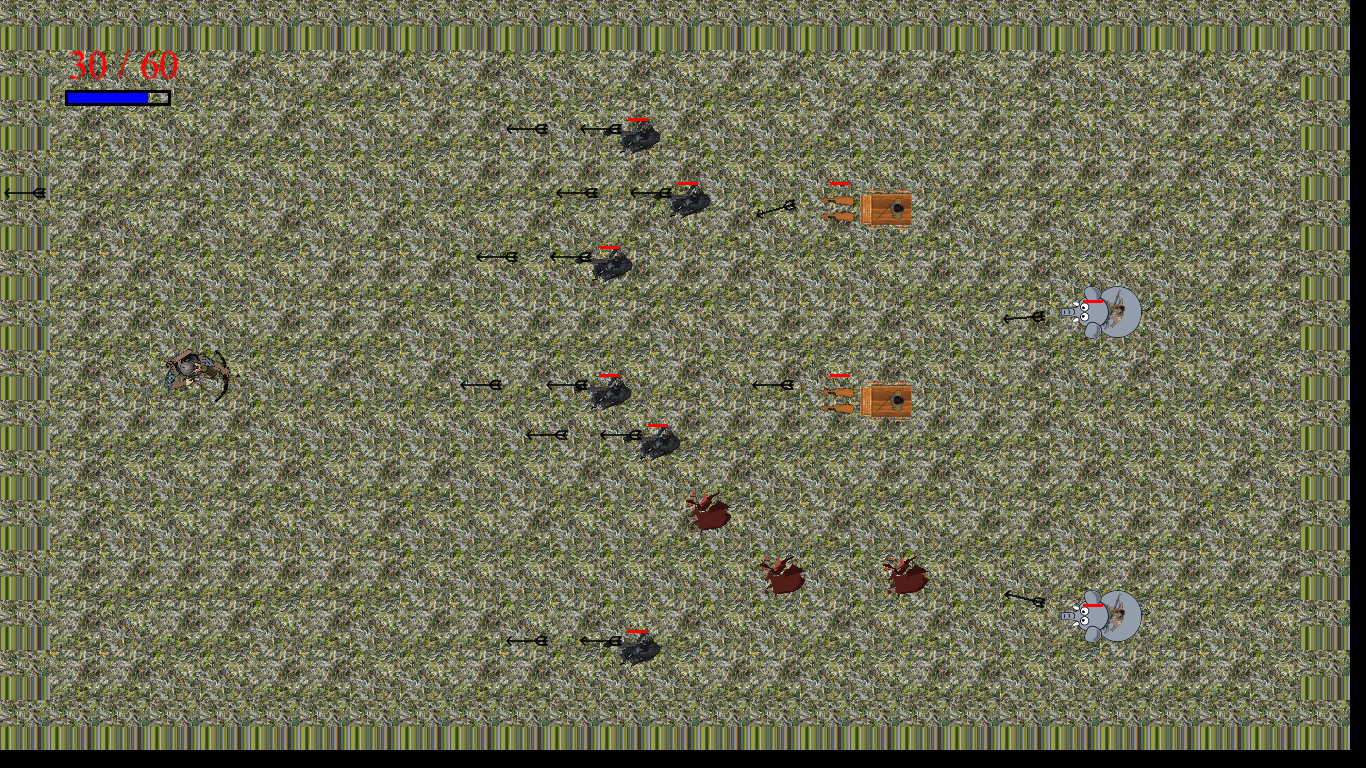
\includegraphics[width = \textwidth]{sec/pdf/level 8}
	\caption{Generalized Block Diagram}
\end{figure}

\vspace{2cm}
\begin{figure}[h]
	
	\centering
	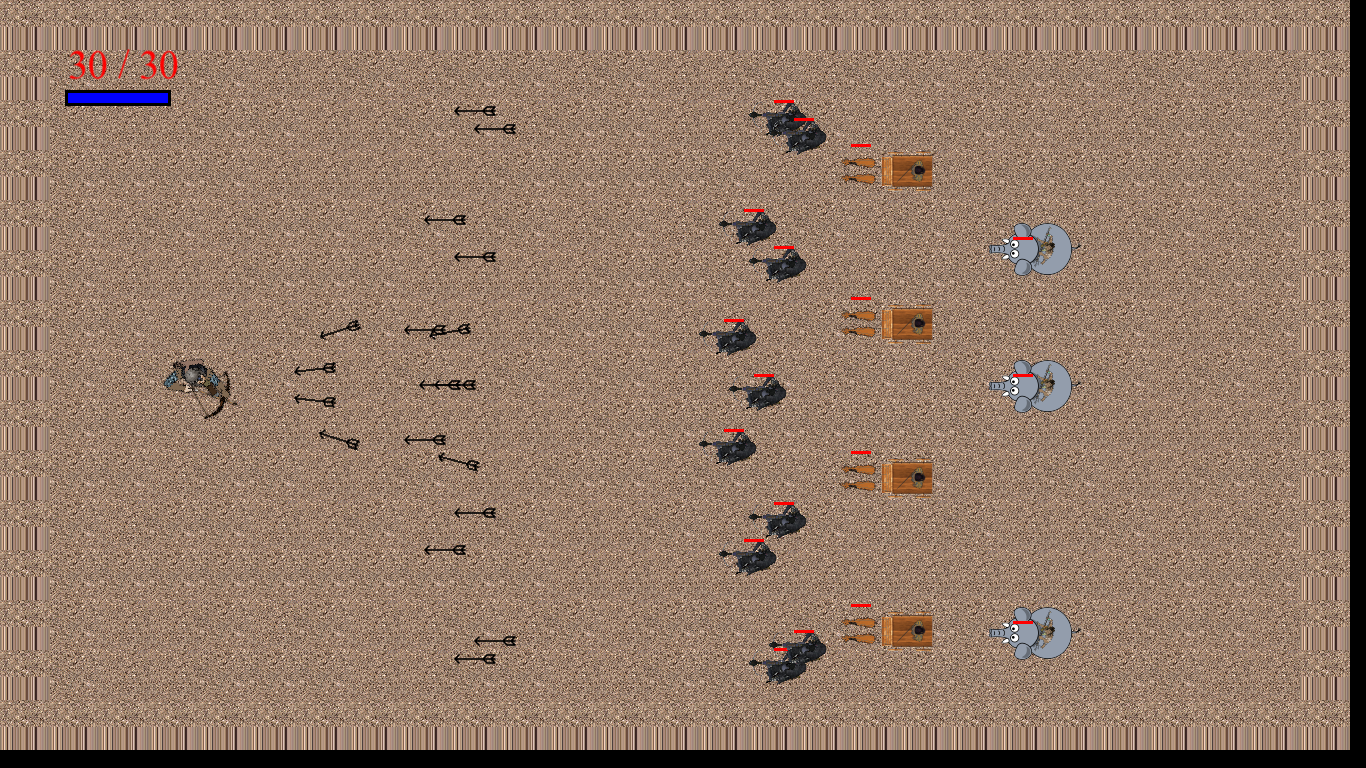
\includegraphics[width = \textwidth]{sec/pdf/level 9}
	\caption{Generalized Block Diagram}
\end{figure}




\newpage